

\section{Maps}
To create a map, a design worked with only a few elements: \cw{VERTEX}, \cw{LINE}, \cw{SIDEDEF}, and \cw{SECTORS}.\\
\par
EXAMPLE HERE\\
\par

The tool to create the maps tool a lot of work. The Doom EDitor was to be called DoomED. Entirely written in Objective-C and running on NeXTStep it benefited from InterfaceBuilder.\\
\par
Since the source code was release in 20XX, we can compare it to the game engine. It turns out there is almost the same amount of code!\\
\par
\tcode{cloc_doomed.txt}

\par
\fullimage{doomed/DoomEd.png}
\par
\fullimage{doomed/all_widgets.png}
\par
\tcode{map.txt}
\fullimage{props/tom.png}
\par
\trivia{The editor startups with a growling imp!}
\par





\section{Map Preprocessor}
\cw{doombsp} processes output from DoomED (XXX files) into XXX, XXX, and XXX. It was released very shorty after Doom shareware on April, 6th 1994. It is a small code base which was critical to the modding community since it enabled enthusiast to compile and inject their own maps into Doom.\\
\par
\tcode{cloc_doombsp.txt}
\par
Trivia: WAD was coined by Tom Halls. "Where's all the data?".\\
\par

\par
\begin{figure}[H]
\centering
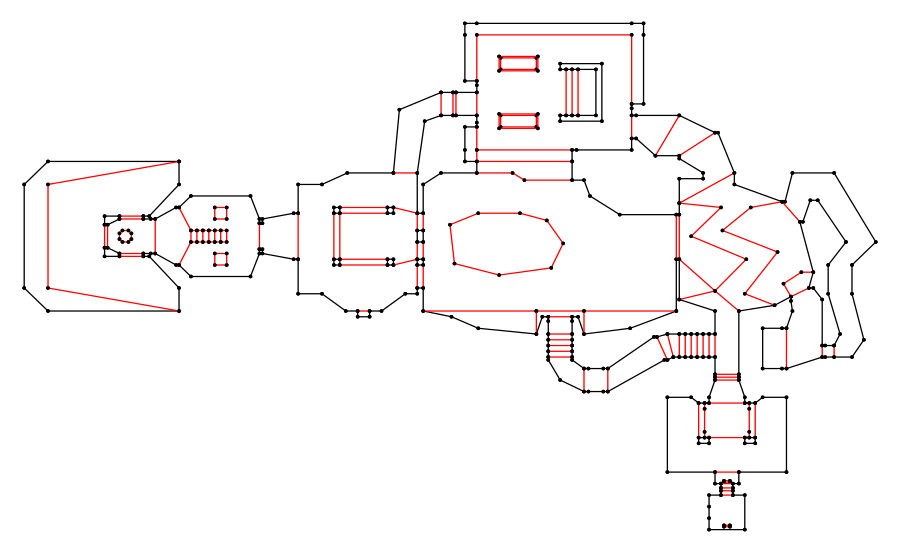
\includegraphics[width=\textwidth]{drawings/E1M1_lines.pdf}
\end{figure}
\par
The map as it is generated via the editor (DoomED) on NextStation.\\
\par
\begin{figure}[H]
\centering
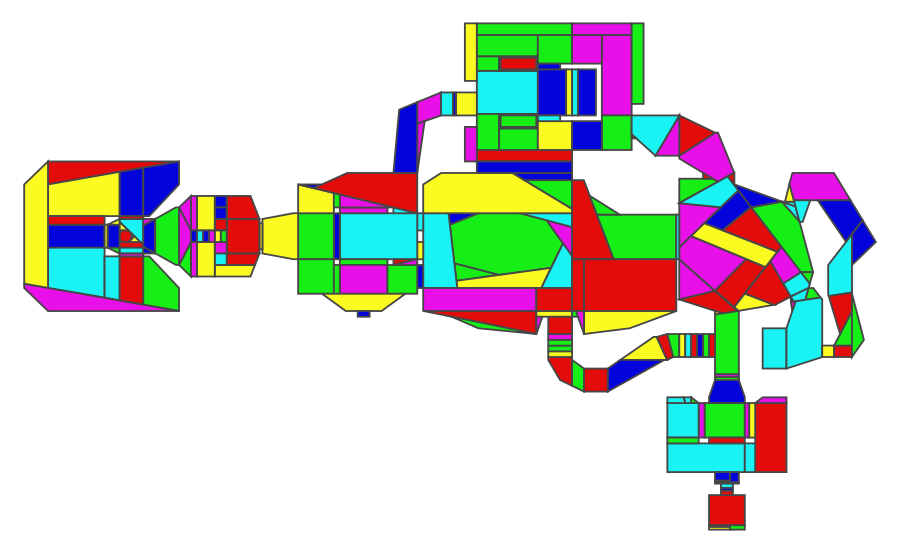
\includegraphics[width=\textwidth]{drawings/E1M1_fab.pdf}
\end{figure}
\par
Binary space partition. Slice all sectors into convex sub-spaces called subsectors.\\
\par
\begin{figure}[H]
\centering
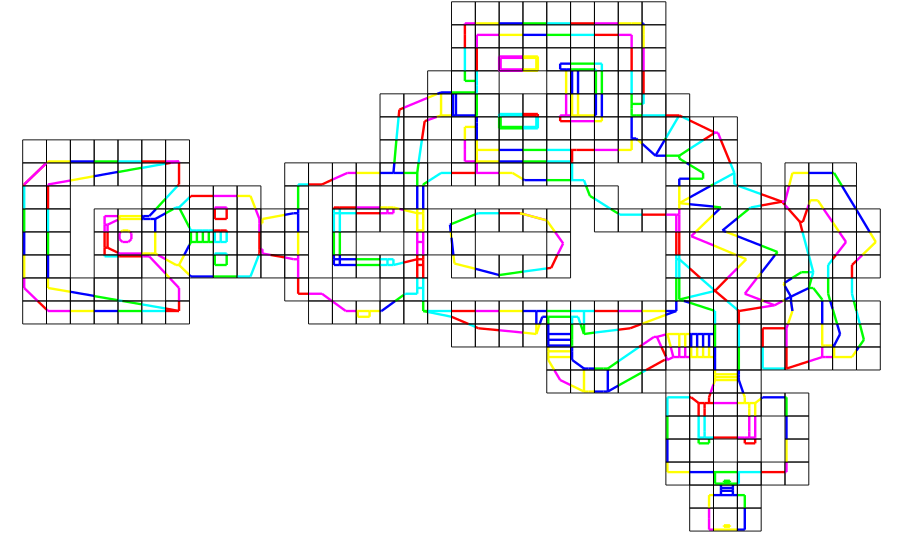
\includegraphics[width=\textwidth]{drawings/E1M1_blockmap.pdf}
\end{figure}
\par
Block based line index.\\
\par
\begin{figure}[H]
\centering
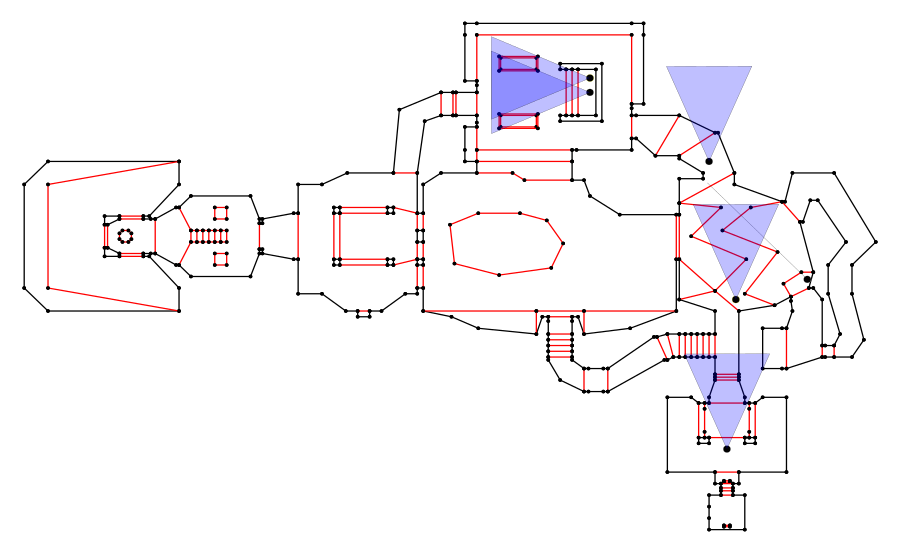
\includegraphics[width=\textwidth]{drawings/E1M1_sides.pdf}
\end{figure}
\par
Reject map based on enemies and monsters line of sight.\\
